La información experimental que puede obtenerse de la estructuras de las 
distintas fases amorfas que se forman durante el ciclado de los electrodos de 
silicio es bastante limitada. Las estructuras de la red o de la interfase son 
inestables y amorfas, lo cual dificulta su caracterización mediante técnicas
experimentales tradicionales. Por ejemplo, la difracción de rayos x permitió
caracterizar la fase cristalina Li$_{15}$Si$_4$ que está presente en el electrodo
cuando este se encuentra completamente cargado ~\cite{obrovac2004}, pero esta 
técnica tiene ciertas limitaciones a la hora de estudiar estructuras amorfas 
que se encuentran en los procesos de carga y descarga. Por otro lado, el análisis
de la función distribución de a pares de Si \textit{ex-situ} de datos de rayos x
hizo posible investigar el orden a corto alcance de las estructuras amorfas
Li$_x$Si ~\cite{key2011} y proponer una explicación al mecanismo de litiación.
Sin embargo, como los elementos livianos como el Li tienen baja sensibilidad a 
los rayos x, las conclusiones están simplificadas a la formación de pequeños 
clusters de Si o de átomos de Si aislados durante la litación, lo cual limita la 
descripción de la estructura a una escala mayor.

Dentro de este contexto, las simulaciones computacionales se posicionan como una
herramienta poderosa para acceder al comportamiento microscópico de las 
estructuras de Li$_x$Si y los cambios que sufren durante la litiación. Actualmente
no existe un único modelo computacional robusto que permita estudiar todos los
diferentes procesos presentes en los electrodos de silicio, por lo que se han 
llevado a cabo distintos esfuerzos en los últimos años para estudiar este sistema.
Donde el mayor obstáculo está relacionado con la naturaleza intrínseca de 
multi-escala del silicio. A pesar de la gran precisión, los estudios de DFT se
encuentran drásticamente limitados en el número de átomos que se pueden utilizar
para modelar las estructuras complejas de las fases litiadas. Una solución a este
problema es utilizar potenciales interatómicos semi-empíricos, para los cuales 
se necesita una parametrización que se robusta y transferible. Como esta 
parametrización esta fuera de los objetivos que plantea esta tesis, en este 
capítulo se utiliza una realizada para un potencial reactivo, introducido en 
la sección \ref{s:reaxff}, para sistemas de Li-Si previamente realizada por Fan 
\textit{et al.} ~\cite{fan2013}, en la cual optimizaron el campo de fuerzas usando 
cálculos de DFT, considerando datos de las energías, distintas geometrías y cargas
de las fases cristalinas de Li, Si y aleaciones de Li-Si. En su trabajo también
utilizaron simulaciones de MD para caracterizar las propiedades mecánicas de
las estructuras amorfas de Li$_x$Si, incluyendo litiación de capa fina, compresión
biaxial, tensión y compresión uniaxial y la tensión que puede soportar el sistema 
antes de deformarse.


\section{Campo de fuerzas}

El campo de fuerzas de Fan \textit{et al.} ha sido ampliamente utilizado en 
simulaciones de MD para estudiar el proceso de litiación de distintas estructuras
de silicio, desde estructuras periódicas a nanoestructuras. Previo a la 
realización del trabajo de este capítulo, se consultó la bibliografía para 
verificar esto y asegurarnos de la transferibilidad del potencial. 

Además de los resultados reportados por Fan \textit{et al.} ~\cite{fan2013}, 
la estructura, el estrés y la difusividad fue estudiada durante la litiación de 
silicio amorfo (a-Si) y silicio cristalino (c-Si) en diferentes orientaciones 
cristalográficas ~\cite{chen2020, kim2015}. Ding \textit{et al.} ~\cite{ding2017} 
reportó la variación de la velocidad de migración en la frontera de fases y la 
difusividad de Li en función del estrés externo aplicado, exponiendo que la 
tensión acelera la razón de litiación, mientras que la compresión la retarda. Kim 
\textit{et al.} ~\cite{kim2014} realizó simulaciones de MD para caracterizar la 
evolución estructural de la frontera de fases entre c-Si, con diferentes planos 
de orientación, con una fase amorfa de litiación máxima. Posteriormente, Fan 
\textit{et al.} ~\cite{fan2018} estudió nanoestructuras, computando la respuesta
mecánica de nanopilares de c-Si en la orientación (111) durante la litiación.
Un trabajo similar, pero para la orientación (100), fue realizado por Cao 
\textit{et al.} ~\cite{cao2019}. Tang \textit{et al.} ~\cite{tang2019} investigó
la evolución y la permanencia de la porosidad de nanocapas de Si durante los 
procesos de litiación y delitiación. Ostadhossein \textit{et al.} 
~\cite{ostadhossein2015} caracterizó la litiación de nanohilos de c-Si y mostró
que este potencial ReaxFF reproduce precisamente las barreras de energía de la
migración de Li obtenidas por DFT, tanto en c-Si como en a-Si.

Este potencial no estuvo sólo limitado al uso en MD, sino que fue aplicado a otros
métodos de simulación, por ejemplo, simulaciones de Monte Carlo en el ensamble
gran canónico fueron realizadas para estudiar un ciclo de litiación y delitiación
de un electrodo de a-Si ~\cite{basu2019}. Trochet y Mousseau ~\cite{trochet2017}
caracterizaron el paisaje energético a concentraciones relativamente bajas de 
impurezas de Li en c-Si, usando una técnica de activación-relajación cinética. 
Kim \textit{et al.} ~\cite{kim2017} desarrolló un algoritmo para investigar la 
respuesta a la delitiación de una capa delgada de silicio recubierta de óxido de 
aluminio. El ReaxFF también fue combinado con otros campos de fuerza, como los
potenciales de Tersoff y Lennard-Jones, para simular la litiación de 
nanopartículas de Si recubiertas con carbono, que permitieron observar una 
correlación entre el crecimiento del estrés y la densidad de carga 
~\cite{zheng2019,zheng2020}. Propiedades mecánicas de interfase Si/SiO$_2$ litiada 
fueron reportadas por Verners y Simone ~\cite{verners2019}. 

El estudio de las propiedades electrónicas no es posible con el uso del ReaxFF ya
que es una de sus limitaciones. Sin embargo, de la discusión previa, puede 
observarse que ha sido capaz de predecir un número importante de propiedades del 
sistema Li-Si.


\section{Configuraciones iniciales}

En este capítulo se estudian las propiedades de las estructuras amorfas Li$_x$Si
para distintos valores de $x$ en el rango que va de 0.21 a 4.2.

\subsection{Estructuras cristalinas}

Algunas estructuras cristalinas de LiSi fueron extraídas del Materials Project
~\cite{materials_project} (mp-1314, mp-672287, mp-569849, mp-29720) y utilizadas 
como estados iniciales. Las celdas primitivas de las estructuras cristalinas se
muestran en la figura \ref{fig:cristalinas}, donde están en orden creciente de 
concentración de Li, las mismas son Si, LiSi, Li$_{12}$Si$_7$, Li$_7$Si$_3$, 
Li$_{13}$Si$_4$, Li$_{15}$Si$_4$, Li$_{21}$Si$_5$ y Li, los enlaces de Si-Si 
están graficados si la distancia entre dos de estos átomos es menor a 2.6\AA. En 
la estructura de LiSi se tiene una remanencia del diamante de Si en los enlaces, 
en Li$_{12}$Si$_7$ hay dos tipos de clusters de átomos de Si, pentagonos y 
estrellas, en Li$_7$Si$_3$ los átomos de Si se encuentran en mancuernas, en 
Li$_{13}$Si$_4$ se tienen las mismas mancuernas más algunos átomos aislados y, 
por último, en Li$_{15}$Si$_{4}$ todos los átomos de Si se encuentran aislados,
al igual que en la Li$_{21}$Si$_5$. Estas estructuras cristalinas fueron 
observadas a temperaturas altas ~\cite{wen1981}, pero no se presentan en el 
funcionamiento de una batería ~\cite{obrovac2004}. Sin embargo, sus posiciones 
pueden tomarse como iniciales para simular a las concentraciones correspondientes.
\begin{figure}
    \centering
    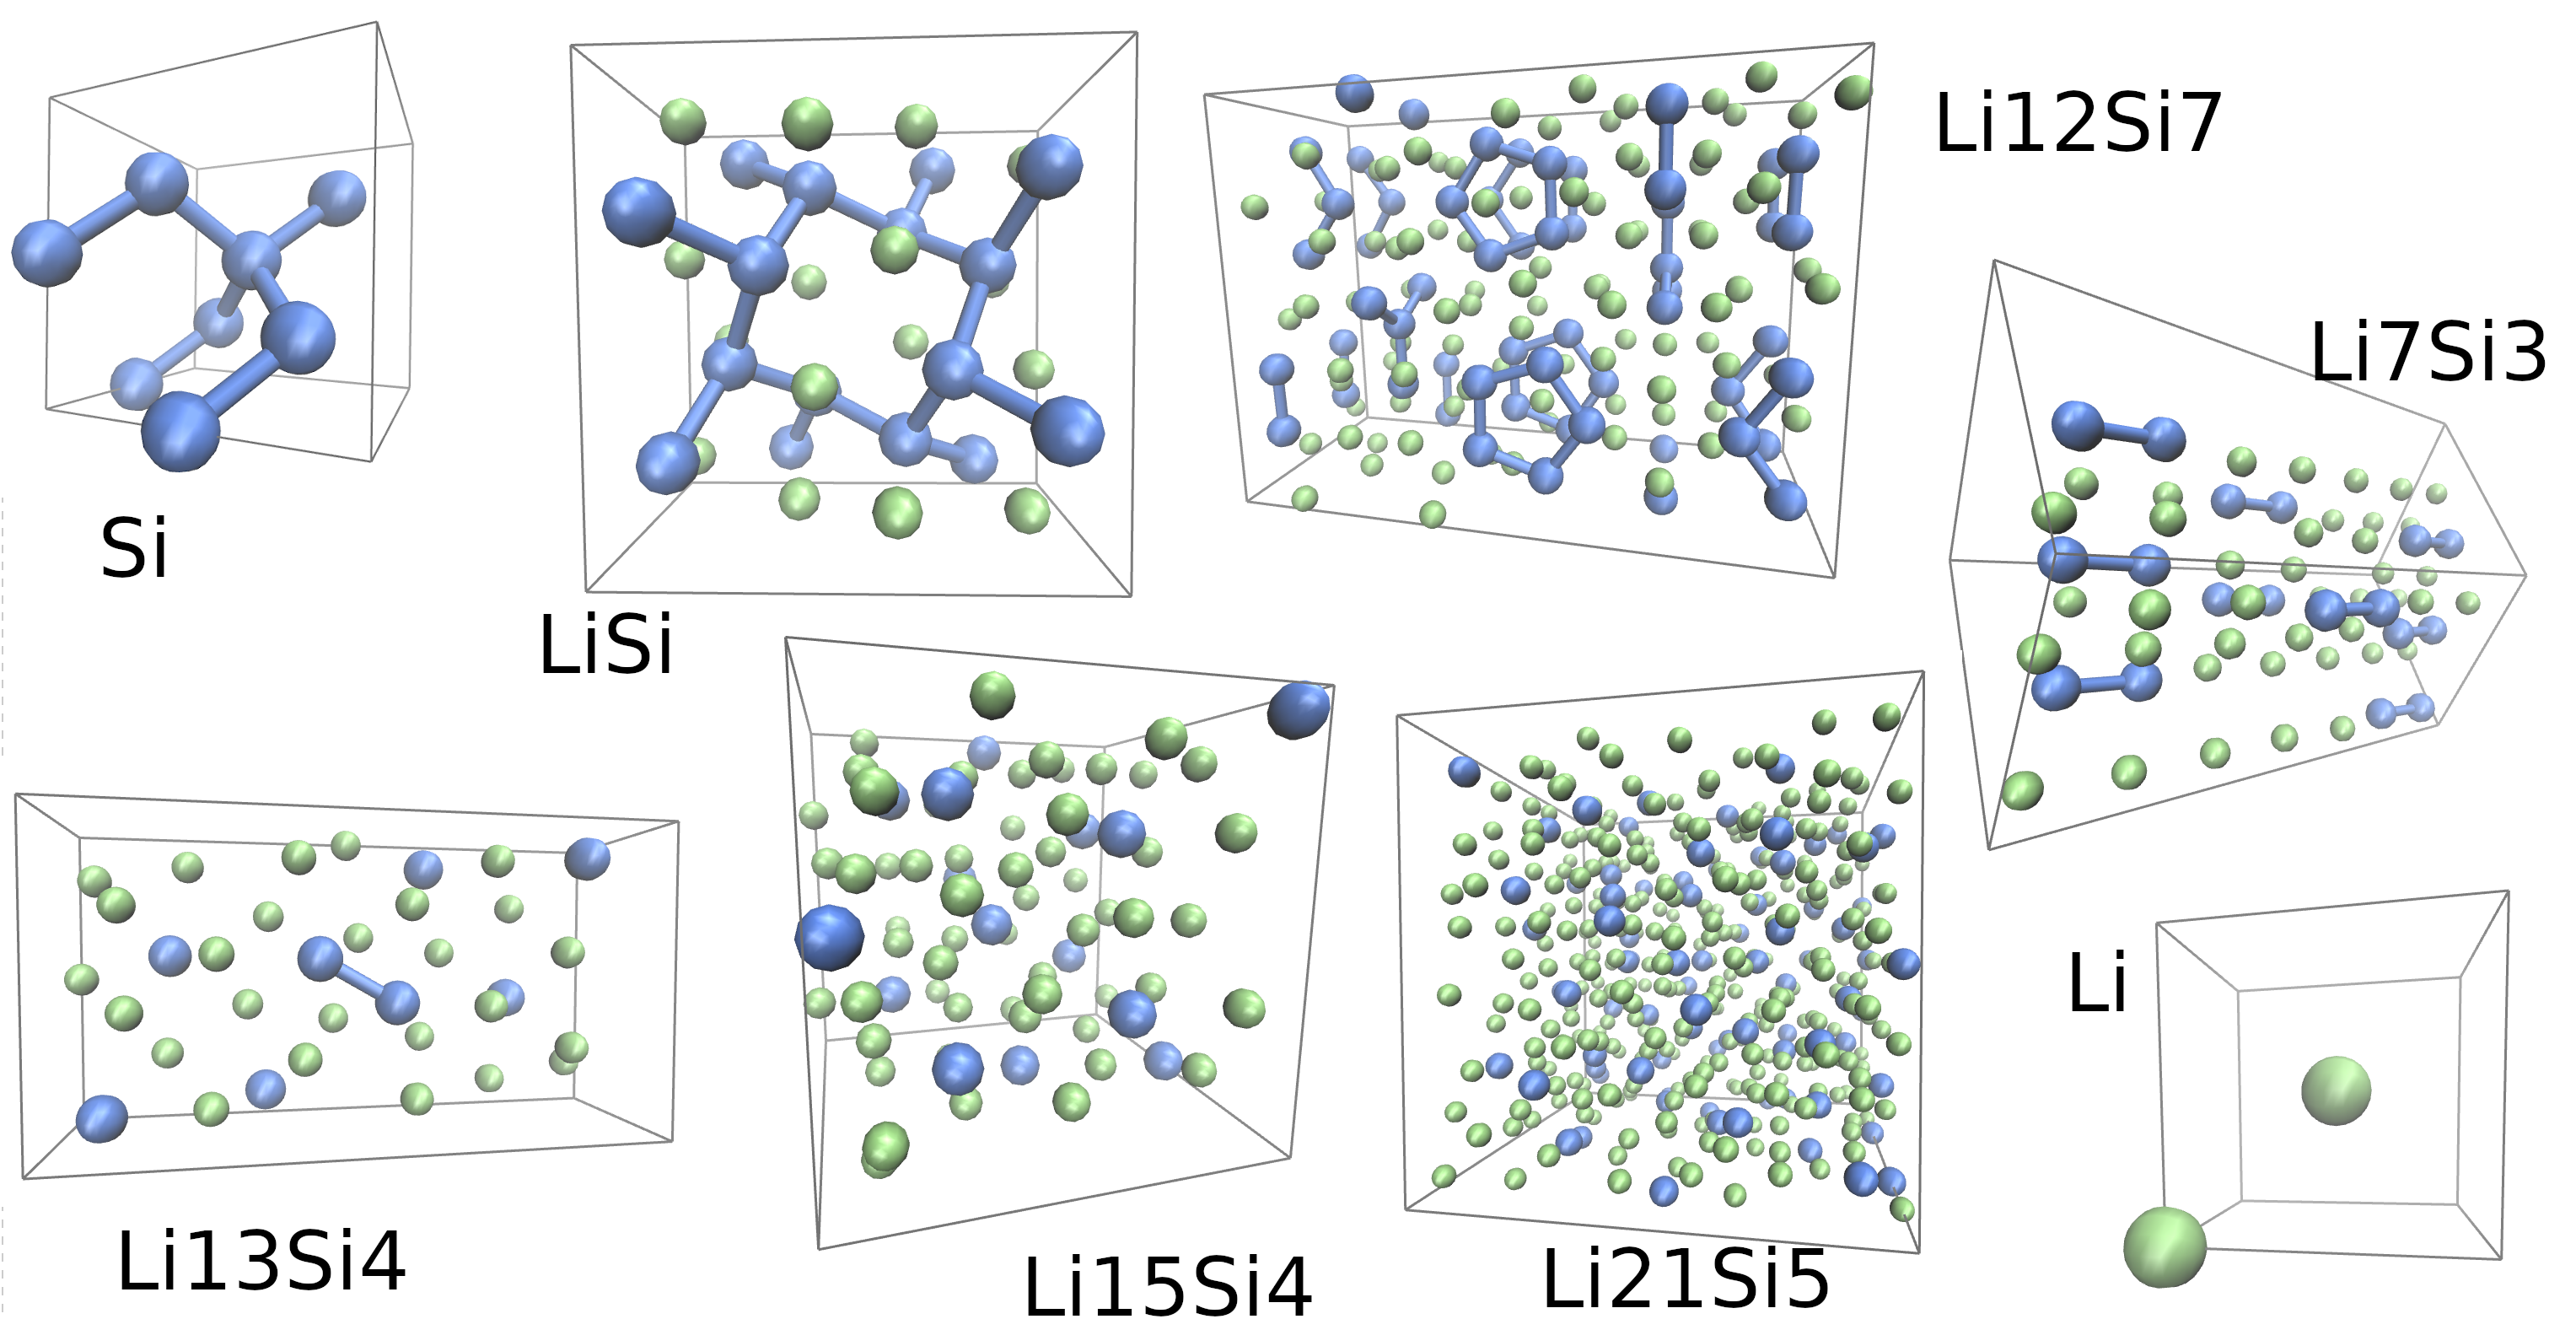
\includegraphics[width=\textwidth]{caracterizacion/cristalinas.png}
    \caption{Estructuras cristalinas de LiSi. Las estructuras no están a escala 
    entre sí. Los átomos de Si se muestran en azul y los de Li en verde, mientras
    que la celda periódica en gris.}
    \label{fig:cristalinas}
\end{figure}

\subsection{Protocolo de delitiación}

Para obtener configuraciones iniciales para valores de $x$ distintos a los de las 
cristalinas se siguió un protocolo de delitiación en el cual se selecciona la 
estructura cristalina más cercana con un valor de $x$ superior al deseado,
se le extrae un átomo de Li de manera aleatoria y se realiza una dinámica en el 
ensamble NPT durante 2 ps para relajar el volumen. Para estas simulaciones se 
utilizó el termostato de Nosé-Hoover ~\cite{nose1984a, nose1984b, hoover1985} a
300.0 K y un barostato a 0.0 atm con un paso temporal de 1 fs utilizando el
software \path{LAMMPS} ~\cite{lammps1, lammps2}. La extracción del átomo de Li y
la simulación en el ensamble NPT fueron repetidas hasta alcanzar una concentración
deseada. Por último, la estructura con la menor presión absoluta fue seleccionada
como estado inicial para la exploración acelerada de mínimos locales que se 
introduce en la siguiente sección.


\section{Exploración acelerada de mínimos locales}

Las simulaciones de MD tienen un gran poder predictivo para el estudio de 
procesos presentes en las baterías de litio, sin embargo, las escalas de tiempo
están limitadas de unos pocos ns o $\mu$s. El número de operaciones que se 
necesita para alcanzar las escalas de tiempo de la operación de una batería 
experimental son prohibitivos, incluso considerando el uso de potenciales 
semi-empíricos como el ReaxFF en supercomputadoras. Como consecuencia de esto,
la MD usual no es suficiente para una exploración del espacio de las fases y las
estructuras de Li-Si observadas van a estar cercanas a las configuraciones 
iniciales mientras que en el sistema real probablemente pueden aparecer otras
configuraciones. Un método simple y poderoso para acelerar la exploración de 
mínimos locales en sistemas moleculares es el templado simulado 
~\cite{kirkpatrick1983}, en el cual básicamente se busca mejorar la exploración
del espacio de las fases en simulaciones de MD utilizando temperaturas altas y
luego reduciéndola progresivamente hasta encontrar un mínimo de energía a 
temperatura ambiente. El templado simulado múltiple (MSA, de sus siglas en inglés 
\textit{Multiple simluated annealing}) fue utilizado para explorar y encontrar
distintas estructuras mínimas relevantes cercanas al equilibrio ~\cite{hao2015}.

La presente técnica de simulación, exploración acelerada de mínimos locales (AELM,
de sus siglas en inglés \textit{accelerated exploration of local minima}), es 
similar a la MSA pero en vez de calentar y enfriar lentamente el sistema, se 
utiliza un sesgo en la función de energía potencial para sobrepasar las barrearas
de energía y luego se realiza una minimización local, con algún minimizador local 
como gradientes conjugados o LBFGS, para encontrar el mínimo. Este método permite 
obtener muchas estructuras con energías mínimas relevantes, que son de interés a 
la hora de estudiar electrodos de Li-Si muy ciclados.

Las aleaciones de Li-Si presentan interacciones fuertes entre los átomos que las
conforman, especialmente en el enlace Si-Si donde la energía de enlace es del
orden de $\approx$2 eV ~\cite{wypych2018handbook}. Las barreras de energía 
potencial se espera que sean de ese orden de magnitud, por lo cual un muestreo de 
una MD a temperatura ambiente parece no tener solución. Para explorar ampliamente
las distintas configuraciones del sistema, $\mathbf{r}$, se transforma 
la superficie de energía potencial (PES, de sus siglas en inglés 
\textit{potencial energy surface}), $V(\mathbf{r})$, usando un potencial sesgado
\begin{equation}\label{eq:bias}
    V_b(\mathbf{r}) = V(\mathbf{r}) + (\alpha - 1) V(\mathbf{r}) = \alpha V(\mathbf{r}),
\end{equation}
donde $\alpha$ es el factor de compresión. La ecuación \ref{eq:bias} reduce las
barreras de la PES, por lo cual el tiempo de residencia en estados meta-estables
es menor que en el sistema sin sesgar y la exploración de configuraciones de 
sistemas diferentes es más eficiente y alcanzada en un tiempo de simulación 
razonable. El término $(\alpha - 1) V(\mathbf{r})$ es usualmente referido como 
la \say{función de sesgo}.

La adición de esta función de sesgo a la PES está en la base del método de 
hiper-dinámica (HD), desarrollado por Voter ~\cite{voter1997HD,voter1997method} 
para acelerar la exploración de un sistema sin perder su dinámica. En una 
simulación típica de HD, para recuperar el promedio de alguna propiedad, la 
configuración muestreada son repesadas por un factor $w$ que involucra una función
exponencial y depende del sesgo aplicado. Debido a que este sistema involucra 
cambios grandes en las energías de interacción, comparado con la energía térmica
$k_BT$, lo que implica que la función exponencial en $w$ toma valores muy grandes,
lo que hace que el procedimiento numérico sea inestable y la recuperación de 
la propiedad de interés, como la energía potencial, no sea posible. Ya que este
capítulo se centra en un estudio estructural de los sistemas, podemos descartar
el cálculo del tiempo real evolucionado en la simulación. Además, como el 
funcionamiento de las baterías luego se da a temperatura ambiente, es de esperar
que una vez que se alcanza un mínimo local el sistema explore configuraciones
cercanas a este. Por lo cual se aplica el método de gradientes conjugados (CG)
a cada configuración de la HD y de esa forma se muestrea la multiplicidad de 
estructuras.

Este método de exploración introducido en esta tesis se asemeja al templado
simulado, aunque el objetivo es explorar muchas estructuras diferentes en vez de 
encontrar el mínimo global. El templado simulado fue utilizado anteriormente
con este mismo objetivo, Hao \textit{et al.} utilizó la técnica MSA para obtener
distintas estructuras de mínima energía de péptidos ~\cite{hao2015}. En este 
método AELM se usa HD en vez de temperaturas altas para favorecer la exploración,
y se realizan múltiples minimizaciones por CG en vez de simular un enfriado. 


\section{Resultados}

Las simulaciones aceleradas fueron llevadas a cabo en el ensamble NVT a 300.0 K
con un termostato de Langevin ~\cite{schneider1978} utilizando una versión 
modificada de \path{GEMS} ~\cite{gems}. El tamaño de los sistemas y la cantidad
de estructuras utilizadas para obtener los siguiente resultados se presentan
en la tabla \ref{t:siminfo}.
\begin{table}[h]
    \centering
    \caption{Información del conjunto de datos.}
    % \begin{tabular}{lrrrrrrr}
    \begin{tabular}{lccccccc}
    \hline
    Li$_{x}$Si & N$_{Li}$ & N$_{Si}$ & N$_{estructuras}$ & E$_{mean}$ / N$_T$ [eV] & E$_{std}$ / N$_T$ [eV] & $\sqrt{kT}$ / N$_T$ [eV] \\
    \hline
    Li$_{0.21}$Si & 140 & 667 & 774 & -4.399 & 0.003 & 0.0002 \\
    Li$_{0.62}$Si & 416 & 670 & 1665 & -4.002 & 0.005 & 0.0001 \\
    Li$_{1.25}$Si & 839 & 671 & 1224 & -3.521 & 0.004 & 0.0001 \\
    Li$_{1.71}$Si & 1152 & 672 & 2132 & -3.286 & 0.002 & 0.0001 \\
    Li$_{2.17}$Si & 693 & 319 & 1699 & -3.126 & 0.002 & 0.0002 \\
    Li$_{2.71}$Si & 865 & 319 & 1504 & -2.964 & 0.002 & 0.0001 \\
    Li$_{3.25}$Si & 1040 & 320 & 1464 & -2.856 & 0.003 & 0.0001 \\
    Li$_{3.75}$Si & 1080 & 288 & 2660 & -2.777 & 0.002 & 0.0001 \\
    Li$_{4.20}$Si & 1344 & 320 & 1600 & -2.717 & 0.001 & 0.0001 \\
    \hline
    \end{tabular}
    \label{t:siminfo}
\end{table}

\subsection{Comportamiento electroquímico}

shows the histograms of the minimum energy obtained using the CG method after HD 
simulations with different $\alpha$s for different alloy compositions. From these 
plots, we selected the most suited acceleration factor leading to the minimum 
energy values from which we got the structural properties of the present alloys. 

\subsection{Distribución radial de a pares}
\subsection{Número de coordinación}
\subsection{Interconexión de clusters}
\subsection{Ordenamiento a corto alcance}


\section{Conclusiones del capítulo}
